\documentclass[a4paper,10pt]{report}
\usepackage[utf8]{inputenc}
\usepackage{hyperref}
\usepackage{graphicx}

\setlength{\parindent}{0mm}
\setlength{\parskip}{2mm}
\setlength{\textwidth}{450pt} %Veränderung des Textblocks in Anpassung an den R Zeilenüberhang bei Aufrufswiederholungen
\setlength{\hoffset}{-50pt} % "
\setlength{\topmargin}{-30pt}
\setlength{\textheight}{670pt}

\setcounter{secnumdepth}{3}
\setcounter{tocdepth}{3}

% Title Page
\title{BRAKER2 User Guide}
\author{Katharina J.~Hoff}


\begin{document}
\maketitle

\tableofcontents

\chapter{Introduction}

\section{What is BRAKER2?}

The rapidly growing number of sequenced genomes requires fully automated methods for accurate gene structure annotation. With this goal in mind, we have developed BRAKER1 \cite{braker1}, a combination of GeneMark-ET \cite{GeneMark-ET} and AUGUSTUS \cite{AUGUSTUS}, that uses genomic and RNA-Seq data to automatically generate full gene structure annotations in novel genomes.

However, the quality of RNA-Seq data that is available for annotating a novel genome is variable, and in some cases, RNA-Seq data is not available, at all.

BRAKER2 is an extension of BRAKER1 which allows for \textbf{fully automated training} of the gene prediction tools GeneMark-EX and AUGUSTUS from RNA-Seq and/or protein homology information, and that integrates the extrinsic evidence from RNA-Seq and protein homology information into the \textbf{prediction}.

In contrast to other available methods that rely on protein homology information, BRAKER2 reaches high gene prediction accuracy even in the absence of the annotation of very closely related species and in the absence of RNA-Seq data. 

BRAKER2 can also combine RNA-Seq and protein homology information. This is in an early stage of implementation, though, and will improve with future releases.

\section{Keys to successful gene prediction}

\begin{itemize}
 \item In order to predict genes accurately in a novel genome, the genome should be masked for repeats. This will avoid the prediction of false positive gene structures in repetitive and low complexitiy regions. Repeat masking is also essential for mapping RNA-Seq data to a genome. In case of GeneMark-EX and AUGUSTUS, softmasking (i.e.~putting repeat regions into lower case letters and all other regions into upper case letters) leads to better results than hardmasking (i.e.~replacing letters in repetitive regions by the letter \texttt{N} for unknown nucleotide).
 
 \item Many genomes have gene structures that will be predicted accurately with standard parameters of GeneMark-ET and AUGUSTUS within BRAKER2. However, some genomes have clade-specific features, i.e.~special branch point model in fungi, or non-standard splice-site patterns. Please read the options section \ref{options} in order to determine whether any of the custom options may improve gene prediction accuracy in the genome of your target species.
 
 \item Always check gene prediction results before further usage! You can e.g.~use a genome browser for visual inspection of gene models in context with extrinsic evidence data.
\end{itemize}

\section{Overview of modes for running BRAKER2}

BRAKER2 mainly features semi-unsupervised, extrinsic evidence data (RNA-Seq or protein spliced alignment information) supported training of GeneMark-EX and subsequent training of AUGUSTUS with integration of extrinsic evidence in the final gene prediction step. However, there are now a number of additional pipelines included in BRAKER2. In the following, we give an overview:

\begin{itemize}
 \item genome and RNA-Seq file from the same species (see figure \ref{braker-main}A); this approach is suitable for RNA-Seq libraries with a good coverage of the transcriptome,
 \item genome file and database of proteins that may be of longer evolutionary distance to the target species (see figure \ref{braker-main}B; this approach is suitable if no RNA-Seq data is available, and if not protein data from a very closely related species is available,
 \item genome file and file with proteins of short evolutionary distance (see figure \ref{braker2-sidetrack}D); this approach is suitable if RNA-Seq data is not available and if the reference species is very closely related,
 \item genome and RNA-Seq file and proteins for short evolutionary distance (see figures \ref{braker2-sidetrack}C and \ref{braker2-sidetrack}E). In both cases, GeneMark-ET is trained supported by RNA-Seq data, and the resulting gene predictions are used for training AUGUSTUS. In approach C), protein alignment information is used in the gene prediction step with AUGUSTUS, only. In approach E), protein spliced alignment data is used to complement the training set for AUGUSTUS. The latter approach is in particular suitable if RNA-Seq data does not produce a sufficiently high number of training gene structures for AUGUSTUS, and if a very closely related and already annotated species is available.
\end{itemize}

\begin{figure}
\begin{center}
\begin{tabular}{c c c c }
 A) & 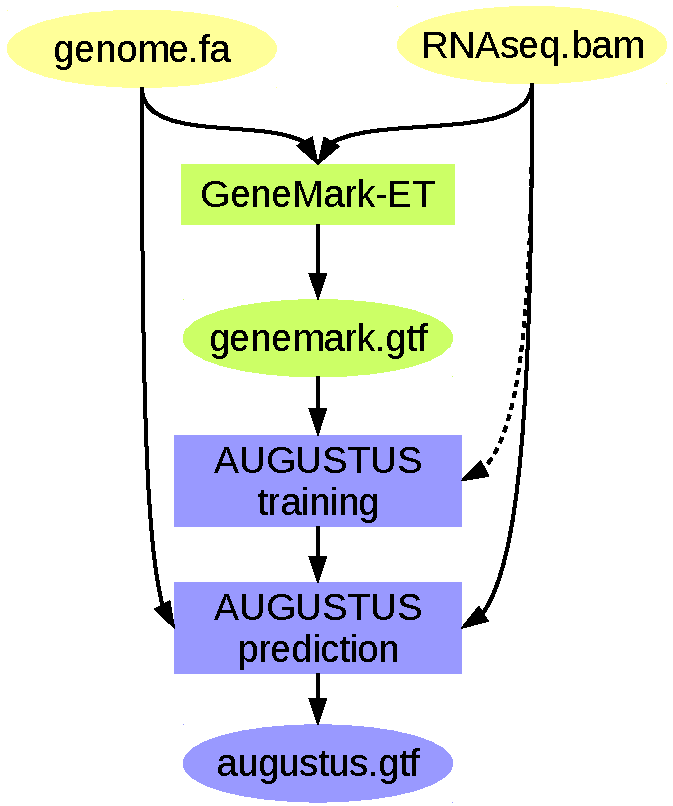
\includegraphics[scale=0.4]{./figs/braker1.pdf} & B) &  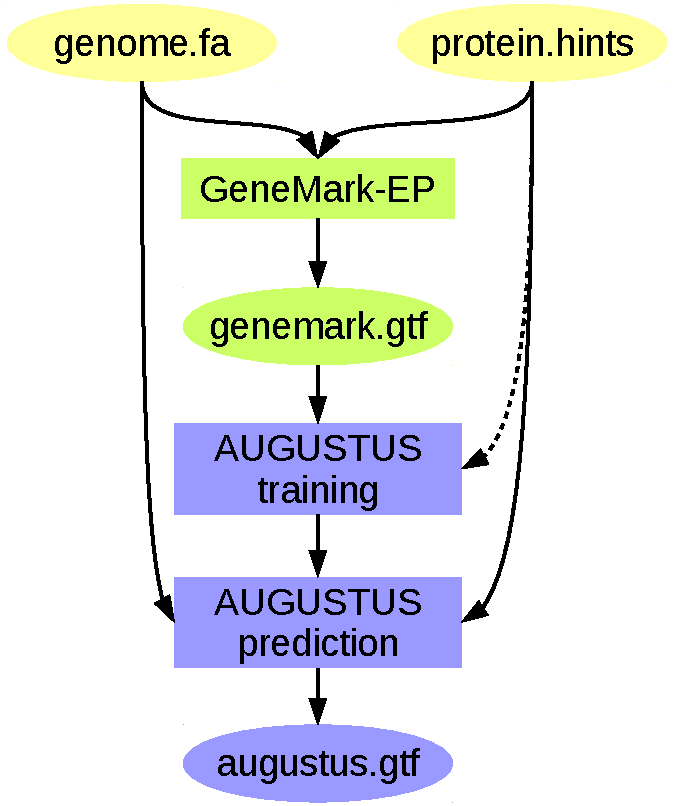
\includegraphics[scale=0.4]{./figs/braker2_ep.pdf}\\
 % braker1.pdf: 323x387 pixel, 72dpi, 11.39x13.65 cm, bb=0 0 323 387
 \end{tabular}
 \caption{BRAKER2 pipeline A) training GeneMark-ET supported by RNA-Seq spliced alignment information, prediction with AUGUSTUS with that same spliced alignment information, B) training GeneMark-EP on protein spliced alignment information, prediction with AUGUSTUS with that same spliced alignment information. Proteins used for B) can be of longer evolutionary distance.\label{braker-main}}
 \end{center}
 \end{figure}

\begin{figure}
\begin{center}
\begin{tabular}{c c c c c c}
 C) & 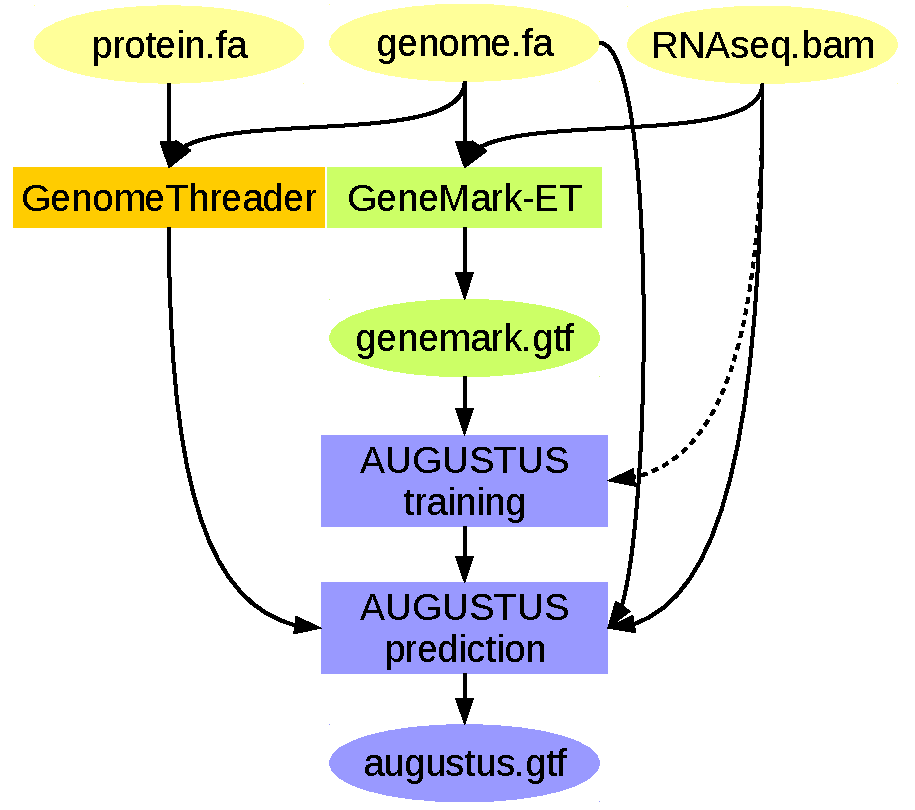
\includegraphics[scale=0.27]{./figs/braker2.pdf} & D) &  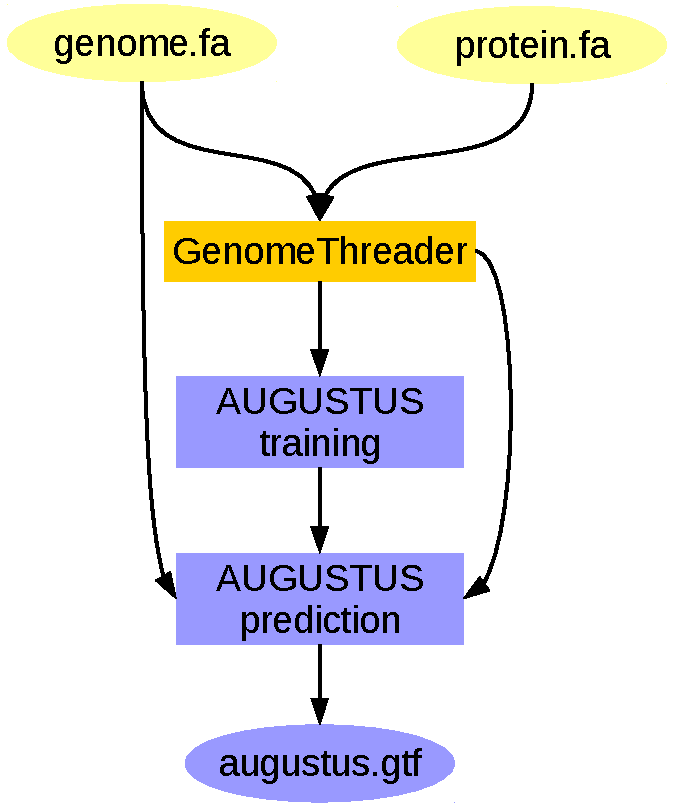
\includegraphics[scale=0.27]{./figs/braker2_gth.pdf} & E) & 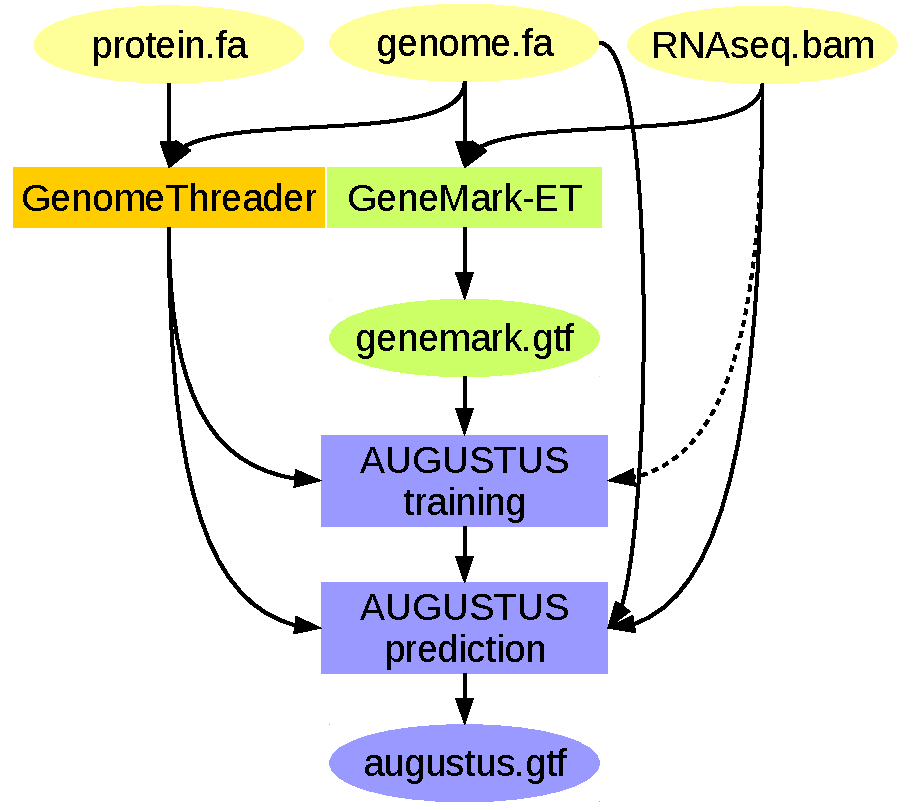
\includegraphics[scale=0.27]{./figs/braker2_train_from_both.pdf}\\
 % braker1.pdf: 323x387 pixel, 72dpi, 11.39x13.65 cm, bb=0 0 323 387
 \end{tabular}
 \caption{BRAKER2 pipeline C) training GeneMark-ET supported by RNA-Seq spliced alignment information, prediction with AUGUSTUS with spliced alignment information from RNA-Seq data and with gene features determined by alignments from proteins of a very closely related species against the target genome, D) training AUGUSTUS on the basis of spliced alignment information from proteins of a very closely related species against the target genome, E) training GeneMark-ET on the basis of RNA-Seq spliced alignment information, training AUGUSTUS on a set of training gene structures compiled from RNA-Seq supported gene structures predicted by GeneMark-ET and spliced alignment of proteins of a very closely related species.\label{braker2-sidetrack}}
 \end{center}
 \end{figure} 
 

\chapter{Installation}

\section{Supported software versions}

At the time of release, this BRAKER2 version was tested with:

\begin{itemize}
\item AUGUSTUS 3.2.2
   \item  GeneMark-EX xxx
   \item  BAMTOOLS 2.4.1
   \item  SAMTOOLS 0.1.19-96b5f2294a
   \item  GenomeThreader 1.1.6
   \item  Spaln 2.3.1
   \item  Exonerate 2.2.0
\end{itemize}

\section{BRAKER2}

\subsection{Perl pipeline dependencies}

BRAKER2 is implemented in Perl. Running BRAKER2 requires a Linux-system with \texttt{bash} and Perl. Furthermore, BRAKER2 requires the following CPAN-Perl modules to be installed:

\begin{itemize}
 \item 		  \texttt{File::Spec::Functions}
				\item \texttt{Hash::Merge}
				\item \texttt{List::Util}
				\item \texttt{Logger::Simple}
				\item \texttt{Module::Load::Conditional}
				\item \texttt{Parallel::ForkManager}
				\item \texttt{POSIX}
				\item \texttt{Scalar::Util::Numeric}
				\item \texttt{YAML}
\end{itemize}

   	On Ubuntu, for example, install the modules with CPANminus: \texttt{cpanm [Module::Name]}.

   BRAKER2 also uses a Perl module \texttt{helpMod.pm} that is not available on CPAN. This module is 
   part of the BRAKER2 release and does not require separate installation.  

\subsection{BRAKER2 components} \label{Executability}

BRAKER2 is a collection of Perl scripts and a Perl module. The main script that will be called in order to run BRAKER2 is \texttt{braker.pl}. Additional Perl components are:

\begin{itemize}
\item \texttt{align2hints.pl}
\item \texttt{filterGenemark.pl}
\item \texttt{filterIntronsFindStrand.pl}
\item \texttt{startAlign.pl}
\item \texttt{helpMod.pm}
\end{itemize}

All Perl scripts (files ending with \texttt{*.pl}) that are part of BRAKER2 must be executable in order to run BRAKER2. This should already be the case if you download BRAKER2 from our website. Executability may be overwritten if you e.g.~transfer BRAKER2 on a USB-stick to anothre computer. In order to check whether required files are executable, run the following command in the directory that contains BRAKER2 Perl scripts:

\begin{verbatim}
ls -l *.pl
\end{verbatim}

The output should be similar to this:

\begin{verbatim}
-rwxr-xr-x 1 braker braker  13802 Jan 12 14:23 align2hints.pl
-rwxr-xr-x 1 braker braker 159944 Jan 16 16:42 braker.pl
-rwxr-xr-x 1 braker braker  21217 Jul  3  2017 filterGenemark.pl
-rwxr-xr-x 1 braker braker   5716 Jul 12  2017 filterIntronsFindStrand.pl
-rwxr-xr-x 1 braker braker  32123 Jan 12 14:23 startAlign.pl
\end{verbatim}

It is important that the \texttt{x} in \texttt{-rwxr-xr-x} is present for each script. If that is not the case, run

\begin{verbatim}
chmod a+x *.pl
\end{verbatim}

in order to change file attributes.

You may find it helpful to add the directory in which BRAKER2 perl scripts reside to 
    your \texttt{\$PATH} environment variable. For a single bash session, enter:

    \begin{verbatim}
    PATH=/your_path_to_braker/:$PATH
    export PATH
    \end{verbatim}
    
To make this PATH modification available to all bash sessions, add the above lines to a startup script (e.g.\texttt{$sim$/.bashrc}).

\section{Bioinformatics software dependencies}

BRAKER2 calls upon various bioinformatics software tools that are not part of BRAKER2. Some tools are obligatory, i.e.~BRAKER2 will not run at all if these tools are not present on your system. Other tools are optional. Please install all tools that are required for running BRAKER2 in the mode of your choice.

\subsection{Mandatory tools}

\subsubsection{GeneMark-EX}

Download GeneMark-EX from \url{http://exon.gatech.edu/GeneMark/license_download.cgi}.
 Unpack and install GeneMark-EX as described in GeneMark-EX's \texttt{README} file.

If already contained in your \texttt{\$PATH} variable, BRAKER2 will guess the location of \texttt{gmes\_petap.pl}, automatically. Otherwise, BRAKER2 can find GeneMark-EX executables either by locating them in an environment variable \texttt{GENEMARK\_PATH}, or by taking a command line argument\\ (\texttt{--GENEMARK\_PATH=/your\_path\_to\_GeneMark-EX/gmes\_petap/}). In order to set the environment variable for your current Bash session, type: 

    \begin{verbatim}
    export GENEMARK_PATH=/your_path_to_GeneMark-ET/gmes_petap/
\end{verbatim}

Add the above lines to a startup script (e.g.~\texttt{$\sim$/.bashrc}) in order to make it available to all bash sessions.\footnote{GeneMark-EX is not a mandatory tool if AUGUSTUS is to be trained from GenomeThreader aligments with the option \texttt{--trainFromGth}.}


\subsubsection{AUGUSTUS}

Download AUGUSTUS from \url{http://bioinf.uni-greifswald.de/augustus/downloads/index.php}.
 Unpack AUGUSTUS and install AUGUSTUS  according to AUGUSTUS \texttt{README.TXT}. 
 
 AUGUSTUS comes with pre-compiled binaries (located in the 
   \texttt{augustus-x.x.x/bin} folder). However, you should compile AUGUSTUS on your own system in order to avoid problems with versions of libraries used by AUGUSTUS. Compilation instructions are provided in the AUGUSTUS \texttt{README.TXT} file
   (\texttt{augustus-x.x.x/README.txt}).

AUGUSTUS consists of \texttt{augustus}, the gene prediction tool, additional C++ tools located in\\ \texttt{augustus/auxprogs} and Perl scripts located in \texttt{augustus/scripts}. Perl scripts must be executable (see instructions in section \ref{Executability} on page \pageref{Executability}). 
   
   The C++ tool \texttt{bam2hints} is an essential component of BRAKER2. Sources are located in \\\texttt{augustus-x.x.x/auxprogs/bam2hints}. Make sure that you compile \texttt{bam2hints} on your system (it should be automatically compiled when AUGUSTUS is compiled, but in case of problems with \texttt{bam2hints}, please read troubleshooting instructions in 
   \texttt{augustus-x.x.x/auxprogs/bam2hints/README}).
   
   Since BRAKER2 is a pipeline that trains AUGUSTUS, i.e.~writes species specific parameter files, BRAKER2 needs writing access to the configuration directory of AUGUSTUS that contains such files  (\texttt{augustus-x.x.x/config/}). If you install AUGUSTUS
   globally on your system, the \texttt{config} folder will typically not be writable by all users. Either make the directory where \texttt{config} resides recursively writable to users of AUGUSTUS, or copy the \texttt{config/} folder (recursively) to a location where users have writing permission. 
   
   AUGUSTUS will locate the \texttt{config} folder by looking for an environment variable \texttt{\$AUGUSTUS\_CONFIG\_PATH}. If the \texttt{\$AUGUSTUS\_CONFIG\_PATH} environment variable is not set, then BRAKER2 will look in 
    the path \texttt{../config} relative to the directory in which it finds an AUGUSTUS executable. Alternatively, you can supply the variable as a command line argument to BRAKER2\\ (\texttt{--AUGUSTUS\_CONFIG\_PATH=/your\_path\_to\_AUGUSTUS/augustus/config/}). We recommend that you export the variable e.g.~for your current bash session:

    \begin{verbatim}
    export AUGUSTUS_CONFIG_PATH=/your_path_to_AUGUSTUS/augustus/config/
    \end{verbatim}

In order to make the variable available to all Bash sessions, add the above line to a startup script, e.g.~\texttt{$\sim$/.bashrc}.
   
   \paragraph{Modification of \texttt{\$PATH}.} Adding adding directories of AUGUSTUS binaries and scripts to your \texttt{\$PATH} variable enables your system to locate these tools, automatically. It is not a requirement for running BRAKER2 to do this, because BRAKER2 will try to guess them from the location of another environment variable (\texttt{\$AUGUSTUS\_CONFIG\_PATH}), or both directories can be supplied as command line arguments to \texttt{braker.pl}, but we recommend to add them to your \texttt{\$PATH} variable. For your current bash session, type:

    \begin{verbatim}
    PATH=:/your_path_to_augustus/bin/:/your_path_to_augustus/scripts/:$PATH
    export PATH
    \end{verbatim}

    For all your BASH sessions, add the above lines to a startup script (e.g.\texttt{$sim$/.bashrc}).

   

\subsubsection{Bamtools}

Download BAMTOOLS (e.g.~\texttt{git clone \url{https://github.com/pezmaster31/bamtools.git}}). Install BAMTOOLS by typing the following in your shell:\\

 \begin{verbatim}
   cd your-bamtools-directory
   mkdir build
   cd build
   cmake ..
   make
 \end{verbatim}

 If already in your \texttt{\$PATH} variable, BRAKER2 will find bamtools, automatically. Otherwise, BRAKER2 can locate the bamtools binary either by using an environment variable \texttt{\$BAMTOOLS\_PATH}, or by taking a command line argument (\texttt{--BAMTOOLS\_PATH=/your\_path\_to\_bamtools/bin/}). In order to set the environment variable e.g.~for your current bash session, type:

    \begin{verbatim}
        export BAMTOOLS_PATH=/your_path_to_bamtools/bin/ 
    \end{verbatim} 

    Add the above line to a startup script (e.g.~\texttt{$\sim$/.bashrc}) in order to set the environment variable for all bash sessions.
    
\subsection{Optional tools}

\subsubsection{Samtools}

Samtools is not required for running BRAKER2 if all your files are formatted, correctly (i.e.~all sequences should have short and unique fasta names). If you are not sure
      whether all your files are fomatted correctly, it might be helpful to have Samtools
      installed because BRAKER2 can automatically fix certain format issues by using Samtools. 

      As a prerequisite for Samtools, download and install \texttt{htslib} (e.g.~ 
      \texttt{git clone \url{https://github.com/samtools/htslib.git}}, follow the \texttt{htslib} documentation for 
      installation).

      Download and install Samtools (e.g. \texttt{git clone \url{git://github.com/samtools/samtools.git}}), 
      subsequently follow Samtools documentation for installation).    

      If already in your \texttt{\$PATH} variable, BRAKER2 will find samtools, automatically. Otherwise, BRAKER2 can find Samtools either by taking a command line argument\\ (\texttt{--SAMTOOLS\_PATH=/your\_path\_to\_samtools/}), or by using an environment variable \texttt{\$SAMTOOLS\_PATH}. For exporting the variable, e.g.~for your current bash session, type:

    \begin{verbatim}
      export SAMTOOLS_PATH=/your_path_to_samtools/
    \end{verbatim}
    
        Add the above line to a startup script (e.g.~\texttt{$\sim$/.bashrc}) in order to set the environment variable for all bash sessions.
\subsubsection{GenomeThreader}

This tool is required, only, if you would like to run protein to genome alignments with BRAKER2 using GenomeThreader. This is a suitable approach if an annotated species of short evolutionary distance to your target genome is available. Download GenomeThreader from \url{http://genomethreader.org/}. Unpack and install according to \texttt{gth/README}.

BRAKER2 will try to locate the GenomeThreader executable by using an environment variable\\\texttt{\$ALIGNMENT\_TOOL\_PATH}. Alternatively, this can be supplied as command line argument \\(\texttt{--ALIGNMENT\_TOOL\_PATH=/your/path/to/gth}).

\subsubsection{Spaln}

This tool is required, only, if you would like to run protein to genome alignments with BRAKER2 using Spaln. This is a suitable approach if an annotated species of short evolutionary distance to your target genome is available. (We recommend the usage of GenomeThreader instad of Spaln.) Download Spaln from \url{http://www.genome.ist.i.kyoto-u.ac.jp/~aln_user}. Unpack and install according to \texttt{spaln/doc/SpalnReadMe22.pdf}.

BRAKER2 will try to locate the Spaln executable by using an environment variable \texttt{\$ALIGNMENT\_TOOL\_PATH}. Alternatively, this can be supplied as command line argument \\(\texttt{--ALIGNMENT\_TOOL\_PATH=/your/path/to/spaln}).

\subsubsection{Exonerate}

This tool is required, only, if you would like to run protein to genome alignments with BRAKER2 using Exonerate. This is a suitable approach if an annotated species of short evolutionary distance to your target genome is available. (We recommend the usage of GenomeThreader instad of Exonerate because Exonerate is comparably slower and has lower specificity than GenomeThreader.) Download Exonerate from \url{https://github.com/nathanweeks/exonerate}. Unpack and install according to \texttt{exonerate/README}. (On Ubuntu, download and install by typing  \texttt{sudo apt-get install exonerate}.)

BRAKER2 will try to locate the Exonerate executable by using an environment variable \\\texttt{\$ALIGNMENT\_TOOL\_PATH}. Alternatively, this can be supplied as command line argument \\(\texttt{--ALIGNMENT\_TOOL\_PATH=/your/path/to/exonerate}).

\chapter{Running BRAKER2}

\section{Different BRAKER2 pipeline modes}

In the following, we describe ``typical'' BRAKER2 calls for different input data types.

\subsection{BRAKER2 with RNA-Seq data (only)}\label{braker1}.

This approach is suitable for genomes of species for which RNA-Seq libraries with a good coverage of the transcriptome are available. The pipeline is illustrated in figure \ref{braker-main}A) on page \pageref{braker-main}.

BRAKER2 can either extract RNA-Seq spliced alignment information from \texttt{bam} files, or it can use such extracted information, directly.

In order to run BRAKER2 with RNA-Seq data supplied as \texttt{bam} file(s) (in case of multiple files, separate them by comma), run:

\begin{verbatim}
   braker.pl --species=yourSpecies --genome=genome.fasta --bam=file1.bam,file2.bam
\end{verbatim}

In order to run BRAKER2 with RNA-Seq spliced alignment information that has already been extracted, run:

\begin{verbatim}
   braker.pl --species=yourSpecies --genome=genome.fasta \
      --hints=hints1.gff,hints2.gff
\end{verbatim}

The format of such a hints file must be as follows (tabulator separated file):

\begin{verbatim}
chrName	b2h	intron	6591	8003	1	+	.	pri=4;src=E
chrName	b2h	intron	6136	9084	11	+	.	mult=11;pri=4;src=E
...
\end{verbatim}

The source \texttt{b2h} in the second column and the source tag \texttt{src=E} in the last column are essential for BRAKER2 to determine whether a hint has been generated from RNA-Seq data. 

\subsection{BRAKER2 with proteins of longer evolutionary distance}

This approach is suitable for genomes of species for which no RNA-Seq libraries are available and for which no closely related and well annotated genome is available. A database of proteins with longer evolutionary distance to the target species may be used in this case. The pipeline is illustrated in figure \ref{gatech} on page \pageref{gatech}.

\begin{figure}
 \centering
 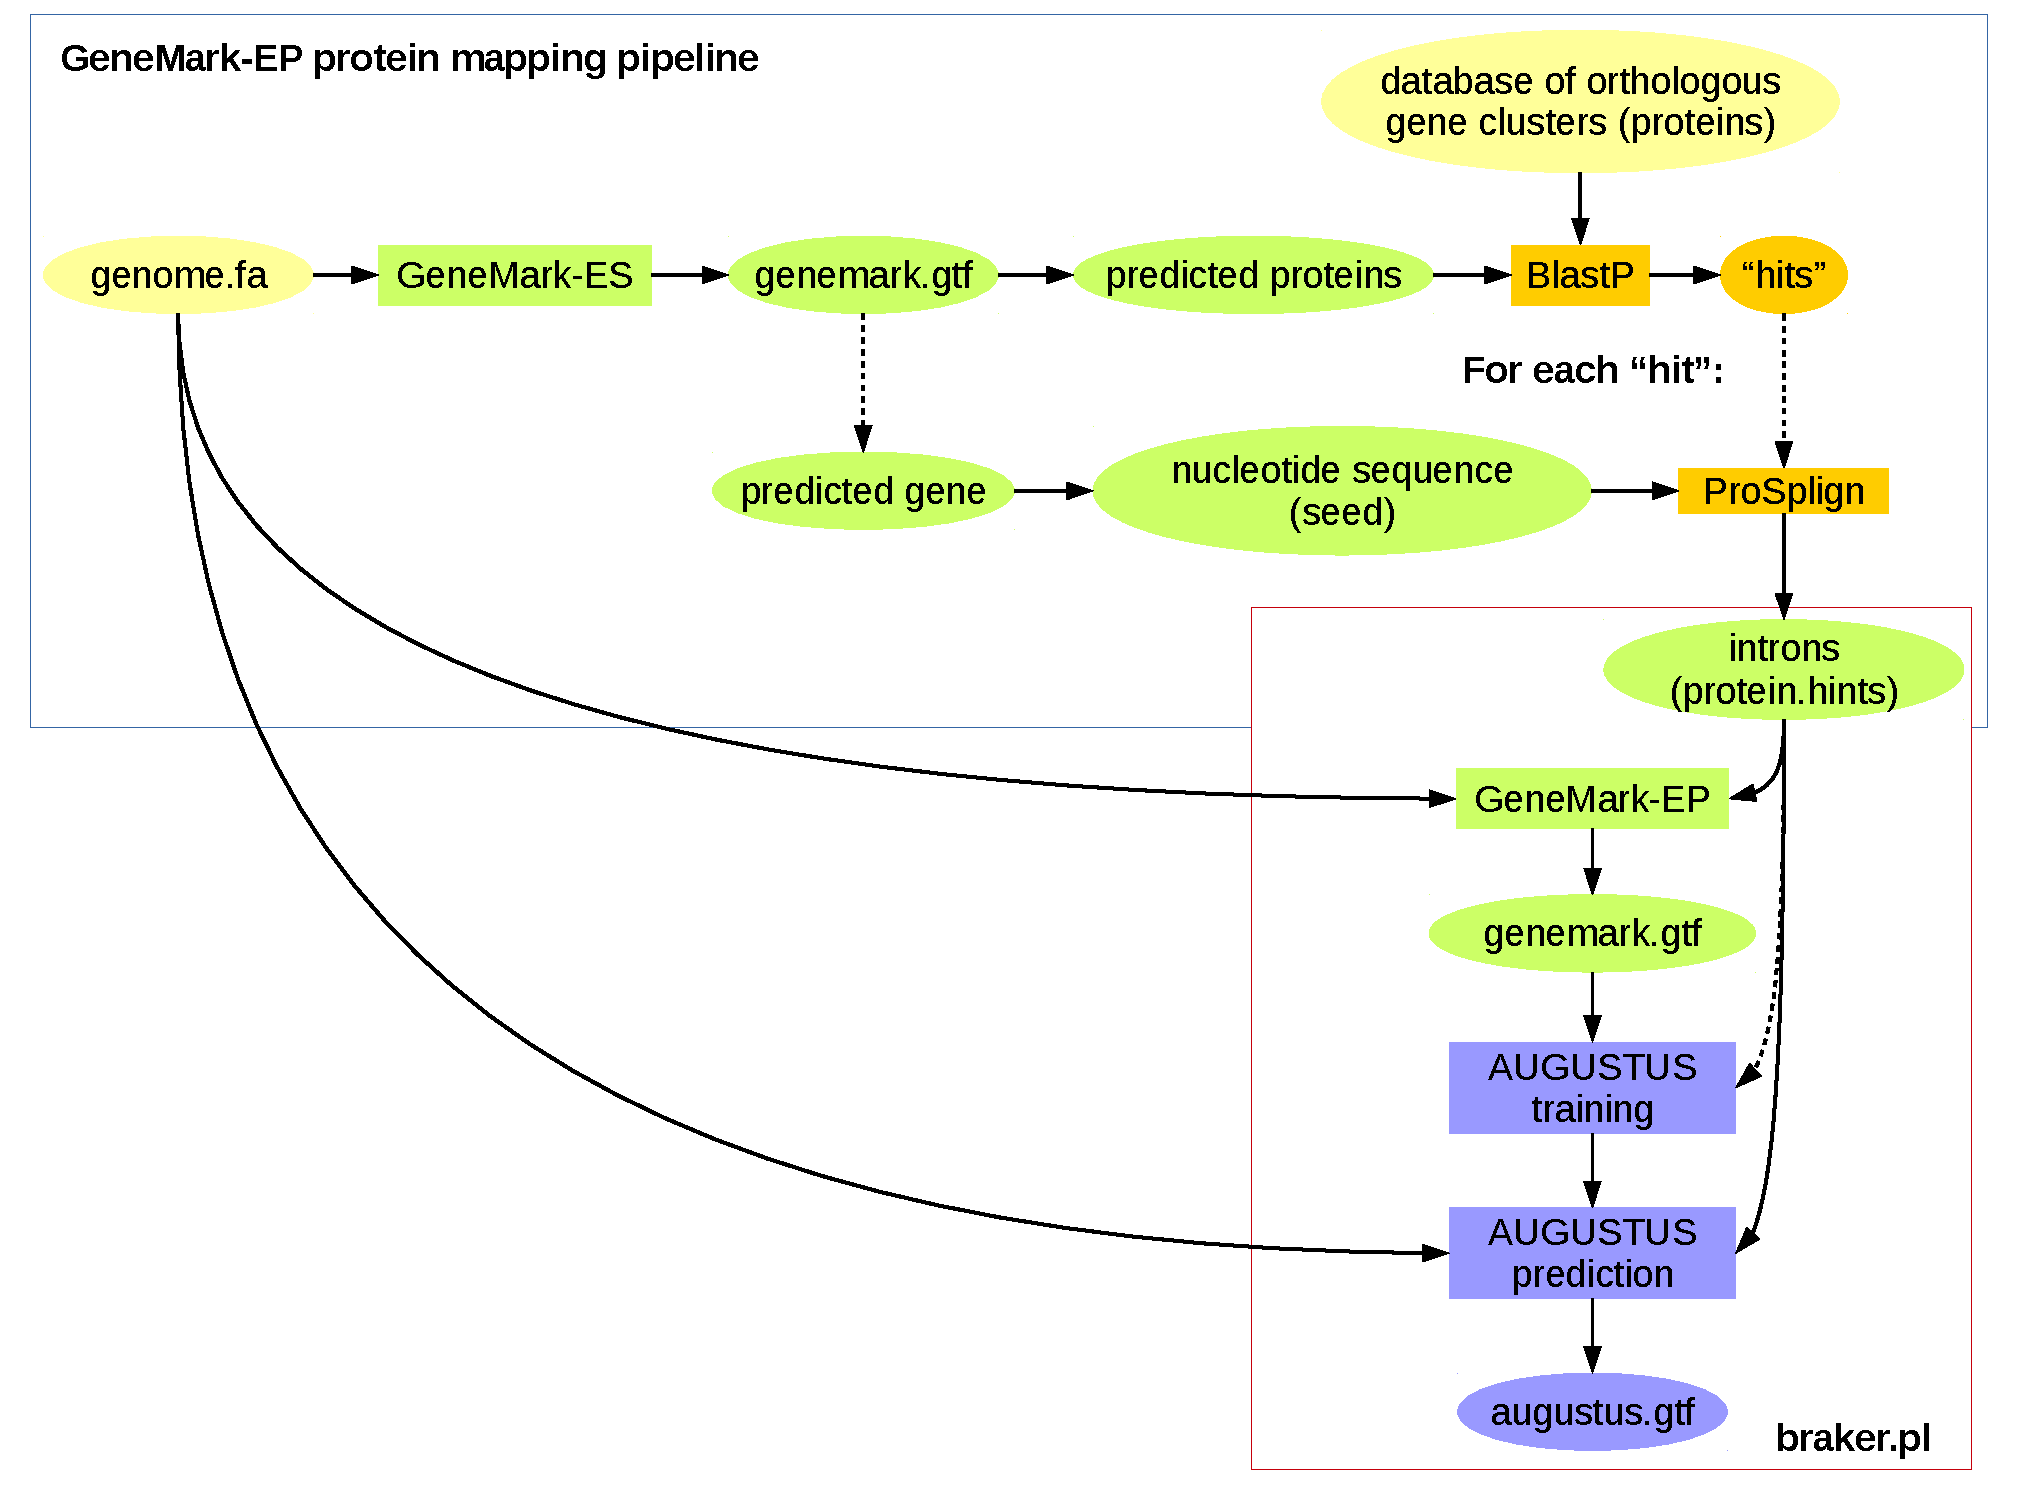
\includegraphics[scale=0.4]{./figs/gatech-prot-pipeline.pdf}
 % gatech-prot-pipeline.pdf: 972x713 pixel, 72dpi, 34.29x25.15 cm, bb=0 0 972 713
 \caption{BRAKER2 and GeneMark-EP protein mapping pipeline.}
 \label{gatech}
\end{figure}

Running BRAKER2 with proteins of longer evolutionary distance requires the preparation of ``protein hints'' before running BRAKER2, itself. Preparing protein hints is in this case not part of BRAKER2 because in contrast to BRAKER2, which can run on a work station with one or multiple cores, the GeneMark-EP specific protein mapping pipeline requires a cluster for execution.

For running BRAKER2 in this mode, type:

\begin{verbatim}
   braker.pl --species=yourSpecies --genome=genome.fasta \
      --hints=hints.gff --epmode
\end{verbatim}

The format of such a hints file must be as follows (tabulator separated file):

\begin{verbatim}
chrName	ProSplign	intron	6591	8003	5	+	.	mult=5;pri=4;src=P
chrName	ProSplign	intron	6136	9084	11	+	.	mult=11;pri=4;src=P
...
\end{verbatim}

The source \texttt{ProSplign} in the second column and the source tag \texttt{src=P} in the last column are essential for BRAKER2 to determine whether a hint has been generated from remote homology protein data. 

\subsection{BRAKER2 with proteins of shorter evolutionary distance}\label{prot-in}

This approach is suitable if RNA-Seq data for the species of the target genome is not available and if a well annotated and very closely related reference species is available. The pipeline is illustrated in figure \ref{braker2-sidetrack}D) on page \pageref{braker2-sidetrack}.

For running BRAKER2 in this mode, type:

\begin{verbatim}
   braker.pl --species=yourSpecies --genome=genome.fasta \
      --prot_seq=proteins.fa --prg=gth --ALIGNMENT_TOOL_PATH=/path/to/gth/binary \
      --trainFromGth
\end{verbatim}

It is possible to generate protein alignments externally, prior running BRAKER2, itself. The compatible command for running GenomeThreader prior running BRAKER2, is:

\begin{verbatim}
   gth -genomic genome.fa  -protein protein.fa -gff3out -skipalignmentout -o gth.aln
\end{verbatim}


In order to use such externally created alignment files, run:

\begin{verbatim}
   braker.pl --species=yourSpecies --genome=genome.fasta \
      --prot_aln=proteins.aln --prg=gth --trainFromGth
\end{verbatim}

It is also possible to run BRAKER2 in this mode using an already prepared hints file. In this case, run:

\begin{verbatim}
   braker.pl --species=yourSpecies --genome=genome.fasta \
      --hints=hints.gff --prg=gth --trainFromGth
\end{verbatim}

Format of the hints file should look like this:

\begin{verbatim}
chrName   gth2h   CDSpart 105984  106633  .     -    .    src=P;grp=FBpp0285205;pri=4
chrName   gth2h   start   106646  106648  .     -    .    src=P;grp=FBpp0285205;pri=4
\end{verbatim}

Supported features are intron, CDSpart, start, stop.

\subsection{BRAKER2 with RNA-Seq and protein data}

BRAKER2 with RNA-Seq and protein data is currently still under development. BRAKER2 currently does not train GeneMark-EX from protein and RNA-Seq data, yet. However, if RNA-Seq data of the target species and protein data of a very closely related reference species are available, BRAKER2 already supports the following to modes.

\subsubsection{Adding protein data of short evolutionary distance to gene prediction step}

This pipeline is illustrated in figure \ref{braker2-sidetrack}C) on page \pageref{braker2-sidetrack}.

In general, add the options

\begin{verbatim}
   --prot_seq=proteins.fa --prg=(gth|exonerate|spaln)
\end{verbatim}

to the BRAKER2 call that is described in section \ref{braker1}. Select one protein alignment tool from GenomeThreader (\texttt{gth}, recommended), Spaln (\texttt{spaln}) or Exonerate (\texttt{exonerate}). Of course, you may also specify the protein information as protein alignment files or hints files as described in section \ref{prot-in} on page \pageref{prot-in}). This may result in a call similar to:

\begin{verbatim}
   braker.pl --species=yourSpecies --genome=genome.fasta --bam=file1.bam,file2.bam \
      --prot_seq=proteins.fa --prg=(gth|exonerate|spaln)
\end{verbatim}

\subsubsection{Extending training gene set with proteins of short evolutionary distance}

If the number of training gene structures identified by RNA-Seq data, only, seems to be too small, you may add training gene structures generated by protein alignments with GenomeThreader to the training gene set. This pipeline is illustrated in \ref{braker2-sidetrack}E) on page \pageref{braker2-sidetrack}.

In general, add the options

\begin{verbatim}
   --prot_seq=proteins.fa --prg=gth --gth2traingenes
\end{verbatim}

to the BRAKER2 call that is described in section \ref{braker1}. This may result in a call similar to:

\begin{verbatim}
   braker.pl --species=yourSpecies --genome=genome.fasta --bam=file1.bam,file2.bam \
      --prot_seq=proteins.fa --prg=gth --gth2traingenes
\end{verbatim}

\section{Description of BRAKER2 command line options}\label{options}

\subsection{\texttt{--help}}                               

Print usage of braker.pl

\subsection{\texttt{--nice}}

Execute (almost) all system calls within braker.pl and its submodules with bash "nice" (default nice value).

\subsection{\texttt{--alternatives-from-evidence=true}}    

Output alternative transcripts based on explicit evidence from hints (default is true).

\subsection{\texttt{--ab\_initio}}

Compute AUGUSTUS \textit{ab initio} predictions in addition to AUGUSTUS predictions with hints (additional output files: \texttt{augustus.ab\_initio.*}.

\subsection{\texttt{--augustus-args=``--some\_arg=bla''}}     
One or several command line arguments to be passed to AUGUSTUS, if several arguments are given, separated by whitespace, i.e.~\texttt{``--first\_arg=sth --second\_arg=sth''}. 
    
\subsection{\texttt{--AUGUSTUS\_CONFIG\_PATH=/path/}}
Set path to config directory of AUGUSTUS (if not specified as 
                                         environment variable). BRAKER1 will assume that the directories
                                         ../bin and ../scripts of AUGUSTUS are located relative to
                                         the \texttt{AUGUSTUS\_CONFIG\_PATH}. If this is not the case, please
                                         specify \texttt{AUGUSTUS\_BIN\_PATH} (and \texttt{AUGUSTUS\_SCRIPTS\_PATH} if required).
                                         The Perl commandline argument \texttt{--AUGUSTUS\_CONFIG\_PATH} has higher
                                         priority than the environment variable with the same name.
                                         
\subsection{\texttt{--AUGUSTUS\_BIN\_PATH=/path/}}           Set path to the AUGUSTUS directory that contains binaries, i.e.~
    					 augustus and etraining. This variable must only be set if 
    					 \texttt{AUGUSTUS\_CONFIG\_PATH} does not have \texttt{../bin} and \texttt{../scripts} of
    					 AUGUSTUS relative to its location i.e. for global AUGUSTUS 
    					 installations. BRAKER1 will assume that the directory
    					 \texttt{../scripts} of AUGUSTUS is located relative to the \texttt{AUGUSTUS\_BIN\_PATH}.
If this is not the case, please specify \texttt{AUGUSTUS\_SCRIPTS\_PATH}.

\subsection{\texttt{--AUGUSTUS\_SCRIPTS\_PATH=/path/}}       Set path to AUGUSTUS directory that contains scripts, i.e.~
    				         \texttt{splitMfasta.pl}. This variable most only be set if
    				         \texttt{AUGUSTUS\_CONFIG\_PATH} or \texttt{AUGUSTUS\_BIN\_PATH} do not contains the
    				         \texttt{../scripts} directory of AUGUSTUS relative to their location, i.e.~
    				         for special cases of a global AUGUSTUS installation.
    				         
\subsection{\texttt{--BAMTOOLS\_PATH=/path/to/bamtools}}
Set path to bamtools (if not specified as environment 
variable). Has higher priority than the environment variable.
\subsection{\texttt{--cores}}                              Specifies the maximum number of cores that can be used during 
                                         computation
\subsection{\texttt{--extrinsicCfgFile=file}}              Optional. This file contains the list of used sources for the 
                                         hints and their boni and mali. If not specified the file ``extrinsic.cfg'' 
                                         in the config directory \texttt{\$AUGUSTUS\_CONFIG\_PATH} is copied and adjusted.
\subsection{\texttt{--fungus}}                             GeneMark-EX option: run algorithm with branch point model (most 
                                         useful for fungal genomes)
\subsection{\texttt{--GENEMARK\_PATH=/path/to/gmes\_petap.pl/}}            

Set path to GeneMark-EX (if not specified as environment variable). Has higher priority than environment variable.
\subsection{\texttt{--gff3}}                               Output in GFF3 format.
\subsection{\texttt{--hints=hints.gff}}                    Alternatively to calling braker.pl with a bam file, it is 
                                         possible to call it with a file that contains introns extracted 
                                         from RNA-Seq (or other data) in gff format. This flag also allows the usage
                                         of hints from additional extrinsic sources for gene prediction 
                                         with AUGUSTUS. To consider such additional extrinsic information,
                                         you need to use the flag \texttt{--extrinsicCfgFile} to specify parameters for 
                                         all sources in the hints file
                                         (including the source ``E'' for intron hints from RNA-Seq).
\subsection{\texttt{--optCfgFile=ppx.cfg}}                 Optional custom config file for AUGUSTUS (see \texttt{--hints}).
\subsection{\texttt{--overwrite}}                          Overwrite existing files (except for species parameter files)
\subsection{\texttt{--SAMTOOLS\_PATH=/path/to/samtools}}            Optionally set path to samtools (if not specified as environment 
variable) to fix BAM files automatically, if necessary. Has higher     
                                         priority than environment variable.
\subsection{\texttt{--skipGeneMark-ET}}                    Skip GeneMark-ET and use provided GeneMark-ET output (e.g.~from a
                                         different source) 
\subsection{\texttt{--geneMarkGtf=file.gtf}}               If \texttt{skipGeneMark-ET} is used, braker will by default look in the 
                                         working directory in folder \texttt{GeneMarkET} for an already existing gtf
                                         file. Instead, you may provide such a file from another location.
                                         If \texttt{geneMarkGtf} option is set, skipGeneMark-ET is automatically also set.
\subsection{\texttt{--skipOptimize}}                       Skip optimize parameter step for AUGUSTUS (not recommended).
\subsection{\texttt{--rounds}}                             The number of optimization rounds used in \texttt{optimize\_augustus.pl} (default 5).

\subsection{\texttt{--skipAllTraining}}                    Skip GeneMark-EX (training and prediction), skip AUGUSTUS training,
                                         only runs AUGUSTUS with pre-trained and already
                                         existing parameters (not recommended). Hints from input are still generated.
                                         This option automatically sets \texttt{--useexisting} to true.
    \subsection{\texttt{--softmasking}}                        Softmasking option for soft masked genome files. Set to 'on' or '1'. Recommended to use this option!
    \subsection{\texttt{--species=sname}}                      Species name. Existing species will not be overwritten. 
                                         Uses Sp\_1 etc., if no species is assigned.                          
    \subsection{\texttt{--useexisting}}                        Use the present config and parameter files if they exist for 
                                         'species'.
    \subsection{\texttt{--workingdir=/path/to/wd/}}            Set path to working directory. In the working directory results
                                         and temporary files are stored.
    \subsection{\texttt{--filterOutShort}}                     It may happen that a ``good'' training gene, i.e.~one that has intron
                                         support from RNA-Seq in all introns predicted by GeneMark, is in fact
                                         too short. This flag will discard such genes that have supported introns
                                         and a neighboring RNA-Seq supported intron upstream of the start codon 
                                         within the range of the maximum CDS size of that gene and with a 
                                         multiplicity that is at least as high as 20\% of the average intron 
                                         multiplicity of that gene.
    \subsection{\texttt{--crf}}                                Execute CRF training for AUGUSTUS; resulting parameters are only kept for
                                         final predictions if they show higher accuracy than HMM parameters. This increases runtime!
    \subsection{\texttt{--prot\_seq=prot.fa}}                   A protein sequence file in multiple fasta format. This file will be used
                                         to generate protein hints for AUGUSTUS by running one of the three
                                         alignment tools Exonerate (\texttt{--prg=exonerate}), Spaln (\texttt{--prg=spaln}) or 
                                         GenomeThreader (\texttt{--prg=gth}). Default is GenomeThreader if the tool is not 
                                         specified.
                                         Currently, hints from proteins are only used in the prediction step with
                                         AUGUSTUS. 
    \subsection{\texttt{--prot\_aln=prot.aln}}                  Alignment file generated from aligning protein sequences against the 
                                         genome with either Exonerate (\texttt{--prg=exonerate}), or Spaln (\texttt{--prg=spaln}), or
                                         GenomeThreader (\texttt{--prg=gth}).
                                         
                                         To prepare alignment file, run Spaln2 with the following command:
                                         
                                         \begin{verbatim}
   spaln -O0 ... > spalnfile
                                            \end{verbatim}
                                            
                                         To prepare alignment file, run Exonerate with the following command:
                                         
                                         \begin{verbatim}
   exonerate --model protein2genome --showtargetgff T ... > exfile
                                            \end{verbatim}
                                            
                                         To prepare alignment file, run GenomeThreader with the following command:
                                         
                                         \begin{verbatim}
   gth -genomic genome.fa  -protein protein.fa -gff3out -skipalignmentout ... -o gthfile
                                         \end{verbatim}
                                         
                                         A valid option \texttt{prg=...} must be specified in combination with 
                                         \texttt{--prot\_aln}. Generating tool will not be guessed.
                                         Currently, hints from proteins are only used in the prediction step with
                                         AUGUSTUS.
    \subsection{\texttt{--prg=gth|exonerate|spaln}}            Alignment tool \texttt{gth} (GenomeThreader), \texttt{exonerate} (Exonerate) or Spaln2
                                         (\texttt{spaln}) that will be used to generate protein alignments that will be the 
                                         basis for hints generation for gene prediction with AUGUSTUS (if specified
                                         in combination with \texttt{--prot\_seq}) or that was used to externally
                                         generate an alignment file with the commands listed in description of 
                                         \texttt{--prot\_aln} (if used in combination with \texttt{--prot\_aln}).
    \subsection{\texttt{--ALIGNMENT\_TOOL\_PATH=/path/to/tool}}  Set path to alignment tool (GenomeThreader, Spaln, or Exonerate) if not 
                                         specified as environment variable. Has higher priority than environment
                                         variable.
    \subsection{\texttt{--gth2traingenes}}                     Generate training gene structures for AUGUSTUS from GenomeThreader
                                         alignments. (These genes can either be used for training AUGUSTUS
					 alone with \texttt{--trainFromGth}; or in addition to GeneMark-ET training genes if 
					 also a bam-file is supplied.)
    \subsection{\texttt{--trainFromGth}}                       No GeneMark-Training, train AUGUSTUS from GenomeThreader alignments.
    \subsection{\texttt{--epmode}}                             Run GeneMark-EP with intron hints provided from \texttt{--hints=proteinhints.gff}.
    \subsection{\texttt{--skipGeneMark-EP}}                    Skip GeneMark-EP and use provided GeneMark-EP output (e.g.~provided with
                                         \texttt{--geneMarkGtf=genemark.gtf}.
    \subsection{\texttt{--version}}                            Print version number of \texttt{braker.pl}.                          


\chapter{Output of BRAKER2}

BRAKER2 produces three important output files in the working directory:

\begin{verbatim}
hintsfile.gff             - The extrinsic evidence data extraced from RNAseq.bam and/or protein
                            data. The introns are used for training GeneMark-EX, all features
                            are used for predicting genes with AUGUSTUS. The file
                            is in gff format.
GeneMark-ET/genemark.gtf  - Genes predicted by GeneMark-EX in gtf format (RNA-Seq trained)
GeneMark-EP/genemark.gtf  - Genes predicted by GeneMark-EX in gtf format (Protein trained)
augustus.hints.gff        - Genes predicted by AUGUSTUS with hints from given extrinsic evidence
                            in gtf format

\end{verbatim}

For details about gtf format, see \url{http://www.sanger.ac.uk/Software/formats/GFF/}. A gtf format file
contains one line per predicted exon. Example:

\begin{verbatim}
HS04636   AUGUSTUS initial  966  1017  .    +    0       transcript_id "g1.1"; gene_id "g1";
HS04636   AUGUSTUS internal 1818 1934  .    +    2       transcript_id "g1.1"; gene_id "g1";
\end{verbatim}

The columns (fields) contain: 

\begin{verbatim}
seqname   source  feature  start   end   score   strand   frame  transcript ID and gene ID
\end{verbatim}


\chapter{Example data}


Due to file size, example data for testing BRAKER2 is separately available for download at 
\url{http://bioinf.uni-greifswald.de/augustus/downloads/index.php} and \url{http://exon.gatech.edu/} as archive
\texttt{BRAKER2examples.tar.gz}.

After extraction, test BRAKER2 with the following commands:

1) For usage with RNA-Seq, only (BRAKER1 functionality):

\begin{verbatim}
   perl braker.pl --genome=/path/to/examples/genome.fa --bam=/path/to/examples/RNAseq.bam
\end{verbatim}

2) For usage with RNA-Seq and proteins (BRAKER2 functionaliy, adapt command to aligner of your 
   choice):
   
   
\begin{verbatim}
perl braker.pl --genome=/path/to/examples/genome.fa --bam=/path/to/examples/RNAseq.bam \
   --prot_seq=/path/to/examples/proteins.fa --prg=gth --ALIGNMENT_TOOL_PATH=/path/to/aligner
\end{verbatim}
   
The runtime of this example should be around 46 hours on a 2.27 GHz single CPU.

\chapter{Bug reporting}


If you found a bug, please contact katharina.hoff@uni-greifswald.de .

Information worth mentioning in your bug report:

Check in \texttt{braker/yourSpecies/braker.log} at which step \texttt{braker.pl} crashed.

There are a number of other files that might be of interest, depending on where in the pipeline the
problem occured. Some of the following files will not be present if they did not contain any errors.

\begin{itemize}
 \item  \texttt{braker/yourSpecies/errors/bam2hints.*.stderr} - will give details on a bam2hints crash (step for 
                                                  converting bam file to intron gff file)
 
 \item  \texttt{braker/yourSpecies/hintsfile.gff} - is this file empty? If yes, something went wrong during hints 
                                      generation
                                    - does this file contain hints from source ``b2h'' and of type 
                                      ``intron''? If not: GeneMark-ET will not be able to execute 
                                      properly.
 
 \item  \texttt{braker/yourSpecies/startAlign.stderr} - if you provided a protein fasta file and this file is not
                                          empty, something went wrong during protein alignment
\item    \texttt{braker/yourSpecies/startAlign.stdout} - may give clues on at which point protein alignment went
                                          wrong

 \item  \texttt{braker/yourSpecies/(align\_gth|align\_exonerate|align\_spaln)/*err} - errors reported by the 
																																		 alignment tools 
                                                                     gth/exonerate/spaln

 \item  \texttt{braker/yourSpecies/errors/GeneMark-ET.stderr} - errors reported by GeneMark-ET
 \item  \texttt{braker/yourSpecies/errors/GeneMark-ET.stdout} - may give clues about the point at which errors in
                                                  GeneMark-ET occured

 \item  \texttt{braker/yourSpecies/GeneMark-ET/genemark.gtf} - is this file empty? If yes, something went wrong 
                                                 during executing GeneMark-ET

 \item  \texttt{braker/yourSpecies/GeneMark-ET/genemark.f.good.gtf} - is this file empty? If yes, something went
                                                        wrong during filtering GeneMark-ET genes 
                                                        for training AUGUSTUS
 
 \item  \texttt{braker/yourSpecies/genbank.good.gb} - try a ``grep -c LOCUS genbank.good.gb'' to determine the 
                                        number of training genes for training AUGUSTUS, should not
                                        be low

 \item  \texttt{braker/yourSpecies/errors/firstetraining.stderr} - contains errors from first iteration of 
                                                     training AUGUSTUS
 \item  \texttt{braker/yourSpecies/errors/secondetraining.stderr} - contains errors from second iteration of
                                                      training AUGUSTUS
   \item \texttt{braker/yourSpecies/errors/optimize\_augustus.stderr} - contains errors optimize\_augustus.pl 
                                                        (additional training set for AUGUSTUS)

 \item  \texttt{braker/yourSpecies/errors/augustus*.stderr} - contain AUGUSTUS execution errors

\end{itemize}


\bibliographystyle{apalike}
\bibliography{refs}

\end{document}          
